%%%%%%%%%%%%%%%%%%%%%%%%%%%%%%%%%%%%%%%%%
% Large Colored Title Article
% LaTeX Template
% Version 1.1 (25/11/12)
%
% This template has been downloaded from:
% http://www.LaTeXTemplates.com
%
% Original author:
% Frits Wenneker (http://www.howtotex.com)
%
% License:
% CC BY-NC-SA 3.0 (http://creativecommons.org/licenses/by-nc-sa/3.0/)
%
%%%%%%%%%%%%%%%%%%%%%%%%%%%%%%%%%%%%%%%%%

%----------------------------------------------------------------------------------------
%	PACKAGES AND OTHER DOCUMENT CONFIGURATIONS
%----------------------------------------------------------------------------------------

\documentclass[DIV=calc, paper=a4, fontsize=11pt, twocolumn]{scrartcl}	 % A4 paper and 11pt font size

\usepackage{lipsum} % Used for inserting dummy 'Lorem ipsum' text into the template
\usepackage[english]{babel} % English language/hyphenation
\usepackage[protrusion=true,expansion=true]{microtype} % Better typography
\usepackage{amsmath,amsfonts,amsthm} % Math packages
\usepackage[svgnames]{xcolor} % Enabling colors by their 'svgnames'
\usepackage[hang, small,labelfont=bf,up,textfont=it,up]{caption} % Custom captions under/above floats in tables or figures
\usepackage{booktabs} % Horizontal rules in tables
\usepackage{fix-cm}	 % Custom font sizes - used for the initial letter in the document
\usepackage{hyperref}

%====== added by BO 08.07.2016 ======================== 
\usepackage{tcolorbox}
\usepackage{enumitem}
%====== edits by BO from 08.07.2016 down to here ===========

\usepackage{sectsty} % Enables custom section titles
\allsectionsfont{\usefont{OT1}{phv}{b}{n}} % Change the font of all section commands

\usepackage{fancyhdr} % Needed to define custom headers/footers
\pagestyle{fancy} % Enables the custom headers/footers
\usepackage{lastpage} % Used to determine the number of pages in the document (for "Page X of Total")

% Headers - all currently empty
\lhead{}
\chead{}
\rhead{}
% Footers
\lfoot{}
\cfoot{}
\rfoot{\footnotesize Page \thepage\ of \pageref{LastPage}} % "Page 1 of 2"

\renewcommand{\headrulewidth}{0.0pt} % No header rule
\renewcommand{\footrulewidth}{0.4pt} % Thin footer rule

\usepackage{lettrine} % Package to accentuate the first letter of the text
\newcommand{\initial}[1]{ % Defines the command and style for the first letter
\lettrine[lines=3,lhang=0.3,nindent=0em]{
\color{DarkGoldenrod}
{\textsf{#1}}}{}}

%----------------------------------------------------------------------------------------
%	TITLE SECTION
%----------------------------------------------------------------------------------------

\usepackage{titling} % Allows custom title configuration
\newcommand{\HorRule}{\color{DarkGoldenrod} \rule{\linewidth}{1pt}} % Defines the gold horizontal rule around the title
\pretitle{\vspace{-30pt} \begin{flushleft} \HorRule \fontsize{25}{25} \usefont{OT1}{phv}{b}{n} \color{DarkRed} \selectfont} % Horizontal rule before the title
\title{The Minimal Mixed-Member Model} % Your article title
\posttitle{\par\end{flushleft}\vskip 0.5em} % Whitespace under the title
\preauthor{\begin{flushleft}\large \lineskip 0.5em \usefont{OT1}{phv}{b}{sl} \color{DarkRed}} % Author font configuration
\author{B. Osberg} % Your name
\postauthor{\footnotesize \usefont{OT1}{phv}{m}{sl} \color{Black} % Configuration for the institution name
% Your institution

\par\end{flushleft}\HorRule} % Horizontal rule after the title
\date{} % Add a date here if you would like one to appear underneath the title block
%----------------------------------------------------------------------------------------

\begin{document}
%\maketitle % Print the title
\thispagestyle{fancy} % Enabling the custom headers/footers for the first page 

\section*{Summary}
The `Minimal Mixed Member' (MMM) model is put forward, here, as a proposal for electoral reform in the Canadian electoral system because it satisfies the following constraints:

\begin{itemize}
\item Accountability: A personal connection must be preserved between all citizens and a specific MP who represents them.  
\item Every vote must count: Citizens should not be discouraged from voting by thinking that their vote will be made irrelevant because of their location. 
\item Proportionality: Major parties must be able to claim their share of popular support. 
\item  Simplicity: The ballots must be easily understood, and the correspondence between ballots and parliamentary power must be clear and intuitive.
\item  Conservatism: Changes to the existing system should be minimized while satisfying the above criteria, and should have evidence of success in an existing democratic state.
\end{itemize}

MMM fulfills these goals through the following procedure:

\begin{itemize}
\item All voters may fill out a ballot with two votes, for a local candidate and a national party, respectively.
\item All first-ballots are counted to produce a riding representative exactly as in the current first-past-the-post (FPP) system.
\item The second ballots are then counted to determine the fraction of the popular vote each party can claim.
\item The \emph{smallest possible number} of additional seats is then introduced using the D'Hondt method (described in the appendix) so that no party is underrepresented.
\end{itemize}

The latter of these points is where this model differs from the current system in Germany (where seats continue to be filled until there are twice as many MPs as ridings). As such, the dilution of power vested in riding-MPs is minimized,  and individual voters may make their intentions more clear by distinguishing between their preferred local candidate and national party (if any).

Using data from the previous election, approximate projections as to the result such a system would have produced in the 2011 and 2015 elections are provided here.


\begin{figure}[h!]
  \includegraphics[width=0.50\textwidth,clip]{Figs/2011_plus_MMM.png}
  \caption{Projected seat distribution following the 2011 federal election, using actual results in bold (left) alongside projected results of this model from the same electorate in transparency (right). The bar defining majority control is also increased to the dashed line for the larger MMM parliament.
}
\label{fig:hypo_2011_sum}
\end{figure}


\begin{figure}[h!]
  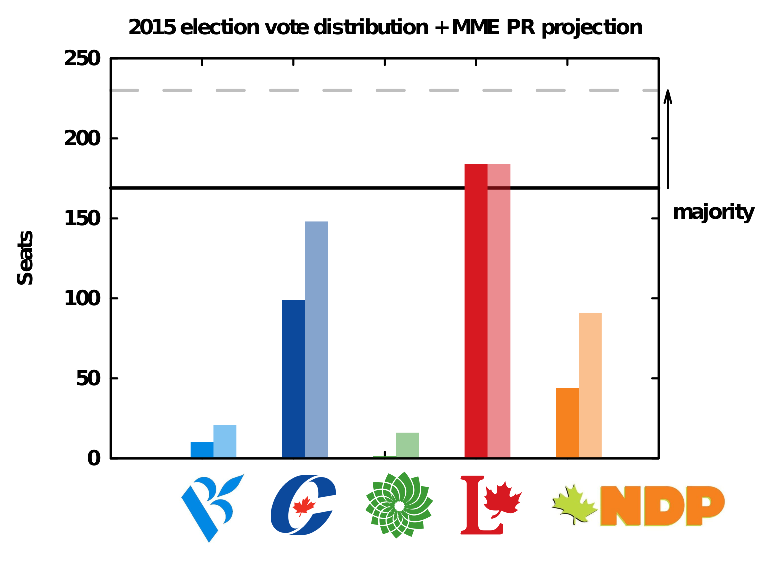
\includegraphics[width=0.50\textwidth,clip]{Figs/Osberg_PR_2015}
  \caption{The same plot as in Fig.~\ref{fig:hypo_2011_sum}, using data from the 2015 election.}
\label{fig:hypo_2015_sum}
\end{figure}

\pagebreak

\maketitle % Print the title
\thispagestyle{fancy} % Enabling the custom headers/footers for the first page 

%----------------------------------------------------------------------------------------
%	ABSTRACT
%----------------------------------------------------------------------------------------

% The first character should be within \initial{}
\begin{abstract}
\textbf{\underline{Abstract:}}
\, Declining voter participation, organized strategic-voting campaigns, public opinion polls\cite{Broadbent_poll}
, and myriad other signals have indicated that Canada's current first-past-the-post (FPP) voting system needs to be changed. 
Accordingly, in the most recent national election campaign, all opposition parties pledged to review the electoral process. 
Although there is clearly a desire for improvement in the way votes are tallied, however, it remains very much unclear as to \emph{how} precisely the system ought to be changed. \\
\, The focus of this paper is to address this problem at a technical level. After briefly reviewing some example voter models from other nations, a specific model (dubbed the `Minimal Mixed-Member', ) is put forward for consideration, having addressed the most common concerns (enumerated here).\\
This model was initially inspired by the mixed-member proportional representation system currently used in Germany, however, by truncating the usual D'Hondt method the number of additional MPs brought into parliament to reach proportionality is minimized (hence, the name).
This method under-representation of parties, while preserving incentive for parties to win local races; it preserves the individual relationship between every voter and an MP; it avoids unnecessary `dilution' of constituency representatives; and it and makes it possible to distinguish between voters' support for local candidates  and national parties. A key feature of this model is that it is conservative in the sense that it modifies our existing system with the minimal set of changes necessary to resolve the most common criticisms of the current system, without introducing unnecessary changes; it fixes only what is broken, and nothing more.
\end{abstract}


%----------------------------------------------------------------------------------------
%	ARTICLE begins
%----------------------------------------------------------------------------------------
\section{Background and Motivation}
\label{sec:BM} 

Assessing the performance of any electoral system requires first clarifying what it is intended to count, and this question is more subtle than it first appears. 
Referenda, for example, generally put a direct question to voters, and a comparison between the ballots for `yes' and `no', at least in principle, establish popular will unambiguously. 
In a general election, however, there are various overlapping preferences that are impossible to disentangle with only a single ballot mark.
Since Canada's FPP system allows voters direct influence only at the riding level, it would seem that the question being posed to voters is as follows:

%--- make a textbox here.
\begin{tcolorbox}[colback=white!5!white,colframe=blue!55!black]
{\textbf{Q1:} } `Which local representative would you ideally like to see represent your riding?'. 
\end{tcolorbox}

Parliament is then selected so as to maximize the number of voters who are provided with this ideal result. 
In practice, however, there are clearly many other questions on voters' minds when they cast their ballot. 
Such questions might include: `Which viable local candidate(s) might you be \emph{satisfied} with?'  or `Which national party do you support?', or `Which national leader would you like to see become prime minister?' 

It has never been entirely clear what priority voters attach to each of these questions during elections. Historically, \textbf{Q1} may have better described the formation of government when geography and limited communications left ridings more isolated.
Advances in telecommunications, for example, have since made national politics more widely accessible. 

Moreover, voter intentions are now influenced by the ready availability of sophisticated statistical pre-election polling. This has increased the importance of `strategic' coordination  between voters' \--in both a formal\cite{Leadnow_environics} and informal sense\footnote{A `strategic  consideration' is defined here as one based on the anticipation of other voters' behaviour}. 

% Thus, it is far from clear that \textbf{(Q1)} captures the voting public's perception of their ballot at election time, and the single `$x$' mark that voters are permitted to make supplies only one bit of information. If we are not even precisely sure of what question is being asked, how can we make sense of the answer?

The distinction between the `ideal' and the `satisfactory' choice is particularly hard to quantify, and often contentious.
Whether or not voters \emph{should} `vote with their hearts' within the current system is a value judgment that will not be addressed here. It should be noted, however, that many strategic voters from the last election were told that 2015 would be the last election under the current system;  their willingness to continue voting strategically is unclear.

More importantly, under the current system citizens of nearly every political persuasion have at some point felt underrepresented \--albeit at different times. It is unlikely that the `joy' of being \emph{over-}represented in certain periods offsets the frustration of under-representation later, and
 national unity can hardly be aided by such stark divisions, even if a kind of \emph{ de facto} proportionality is established on long-term averages. 
Perhaps what can be said at the moment is that various political parties have now had `their turn' to take advantage of the undemocratic peculiarities of our current system and that the time is now ripe to end these disparities and make our system democratic at all times. 

The benefits of such changes can be seen in existing research that `clearly identifies' higher voter turnout rates in voting systems with some form of proportional representation (PR) \cite{Blais}
 across many nations. In a particularly relevant case study, New Zealand was found to have succeeded in `fostering more positive attitudes about the efficacy of voting' as well as an increase in overall turnout during its transition from FPP to PR\cite{NZ_PR_results}
 .

There are some risks, however. Germany demonstrated that some systems of PR can have unintended consequences when it was inconveniently revealed that their PR system allowed \emph{negative} vote weights in some circumstances\cite{Die_Zeit_negative_vote} 
\footnote
{
To briefly summarize: the German system allocated overhang seats (i.e. constituency seats won in excess of popular share) to each state independently, while popular vote share was calculated across the entire country.
In certain situations, a party could win seats that would have been assigned to them anyway (via overhang constituency seats), with little change to its share of the national vote; effectively eliminating their `overhang'. A seat in the Bundestag reserved for proportionality might then be shifted elsewhere, resulting in a net loss of one seat for the party.
This problem arises because of the fixed number of seats in the parliament, and the need for each seat to be assigned to \emph{someone}. However, this quandary prompts the question: if a seat is not necessary to represent a constituency, nor to establish proportionality, then why not eliminate it entirely? We will return to this question in Sec.~\ref{sec:model_proposal}.
}.
This pathological case led to the system being ruled unconstitutional by the courts and the embarrassing technical oversight was removed from the formula. 
Clearly, avoiding such issues in a Canadian system is paramount, however it also serves to highlight a potential peril.
Voting systems are complex, involving millions of participants, and the current system, while imperfect, has worked at least well enough to maintain a peaceful democracy for over a century. The greater tinkering that is done to the electoral system, the greater the chances of unintended consequences. 
Indeed, while a recent report\cite{Broadbent_poll} showed overwhelming support for at least some change to the political system, about half of respondents were wary of \emph{too much} change \--evidently preferring a system that has been tried and tested. As such, keeping change to minimum while resolving specific problems in our existing system will be a principle theme in the following sections.


%------------------------------------------------------------------------------------------------
\section{Defining the Goal}
%------------------------------------------------------------------------------------------------
\label{sec:goal_list}

Here, a coarse list of essential and desirable characteristics in an electoral system are enumerated to serve as guiding principles of the model that will be proposed in Sec.~\ref{sec:model_proposal}.  
\begin{enumerate}
\item \textbf{A personal connection} must be maintained between all citizens and an MP whose role is to represent \emph{them} specifically.   
\item \textbf{Every vote must count} productively. Scenarios in which citizens are discouraged from voting by thinking that their vote will not matter (or, much worse, that it might actively work against their interests) must be eliminated.
\item \textbf{Proportionality} of national support for major groups \--either political parties, or national leaders\-- must be at least approximated within some objective threshold\footnote{
An \emph{exact} mirror of popular support would generally require as many MPs as voters, which is clearly impractical. Rounding, at a minimum, will be necessary.
}. 
\item   \textbf{Simplicity.} The ballot must be sufficiently easy to understand to avoid any widespread difficulty in filling it out. 

\item  \textbf{A clear mandate} should indicate to each MP whether they were elected on their individual merits, or via public support for their party.
\\
and, lastly, 
\item \textbf{Conservatism.} While imperfect, our current democratic system has many advantages; we should change our existing system only as much as is necessary to achieve the above goals, and no more. Changes that \emph{are} proposed to our existing system should have some evidence of success in an existing democracy.
\end{enumerate}

%----------------------------------------------------------------------------------------
%	DIFFERENT PROPOSALS FOR REFORM
%----------------------------------------------------------------------------------------

\section{Alternative Models}
\label{sec:alt_models}

With the list established in Sec.~\ref{sec:goal_list}, we can consider some of the current electoral systems elsewhere in the world and how well they meet our criteria. For example, the \emph{list system}, as used in Israel, produces party representation in proportion to the popular vote; it is easily understood, and it ensures that every vote counts \---all points in its favor. 
The ranking of the party lists, however, is generally determined within the party, leaving candidates no signal as to their individual popularity in any particular riding. Moreover, without separate electoral districts, the connection of voters to a specific MP is eliminated, leading to criticism from such scholars as Enid Lakeman\cite{Lakeman}
.

The single transferable vote (STV) \---as used in Ireland, for example\cite{Irish_howto_vote_doc}
\--- represents something of a compromise between the Israeli and Canadian systems. In Ireland, multi-seat constituencies allow voters to  rank their preferences and if a voter's first choice fails to be elected (or receives such support that additional votes would be superfluous), their vote is transferred to the voter's second preference, and so on. In constituencies with only one seat, this is equivalent to a ranked ballot (and consistent with requirement (1) above). 
Although the Irish balloting process involves some increased complexity in the \emph{counting} process, from each voter's perspective, the concept of ranked preference is easily understood and can be made without the need for strategizing.

Note, however, that this is \emph{not} a form of PR; the STV allows for scenarios in which a single party may receive widespread support across the country, and yet still insufficient support in any specific riding to be awarded any seats. Rather, ranked ballots explicitly incorporate a voters willingness to compromise into their ballot, and maximizes the number of voters who get a representative that they `can live with'.
Altering our voting system in this way would be akin to supplementing question \textbf{(Q1)} from Sec.~\ref{sec:BM} above with the following: 

\begin{tcolorbox}[colback=white!5!white,colframe=blue!55!black]
`\ldots and if your ideal candidate cannot be elected, who \emph{then} would you choose?'. 
\end{tcolorbox}

Part of the appeal of this simple adaptation would be the minimal alteration that would be required to the existing system \--it is merely a matter of gathering additional information from the voters for possible contingencies.

One further note about the STV/ranked ballot deserves mention: It has been argued\cite{Record}
 that the STV would benefit the currently-governing Liberal party since  `centrist' parties are more likely to accumulate second-place votes than parties on either end of the political spectrum. 
Whether such an advantage would be `fair' or `unfair' (i.e. should we consider only voters' `pure' beliefs, or perhaps also their willingness to compromise?) is, again, a value judgment that will not be addressed here. Rather, we will focus on the technical question of whether such an advantage actually exists at all.

While it is impossible to know exactly how many voters are currently voting `with their hearts', it may well be the case that voters who are currently voting `strategically' for centrist candidates will be more likely to risk voting for an underdog if they know that they have an `insurance policy' to fall back on. 
A sufficient shift in first-choice ballots from these risk-averse voters may actually result in surprise upsets with currently `centrist' seats being won by other parties who were superficially thought to have no chance of winning. Given the way ranked ballots are assigned by priority, it remains very much unclear which political party will benefit most from such a system. 

This latter consideration, however, underscores a unique problem of the STV:  there is no obvious mechanism for filtering out small parties to prevent parliament from becoming fragmented. As such, STV could lead to the proliferation of many small parties
(unlike both the list system and  mixed-member models which often use a 5\% `cut-off' in popular support to restrict allocation of proportional seating to `major' parties). 
Moreover, the STV system also falls short of our criteria in two important ways.
First of all: not all votes will `count' in this system. Suppose a voter lives in a riding where a single candidate (regardless of how the voter feels about this candidate) has such overwhelming support as to virtually guarantee victory; or suppose the voter only feels comfortable giving their support to one or two candidates, none of whom have a chance of winning. In either of these cases, the rationale to stay home and not bother voting is similar to our current system. 
Secondly, this system still will not ensure proportionality: It is entirely possible that parties with significant support dispersed across the country will fail to gather sufficient high-priority votes in any specific riding and will still gain few seats overall.  
We are then left with the same problem of disparity between the cumulative national popular vote, and parliamentary representation.
Thus, the STV falls short of requirement (3) in a way that is not easily resolved. 

Nevertheless, criticism of the STV/ranked ballot should not be overstated here; overall, such a model meets most of our requirements and provides a significant set of improvements to our existing system that merit serious consideration. In the following section, however, we will explore another model that satisfies our requirements even more thoroughly.


% --------  German MM ----------------
\subsection{The German Model: A Case Study}
\label{sec:german_model}

Perhaps the electoral system currently in practice in the world that comes closest to satisfying our requirements is found in Germany.

Today German citizens are presented with two votes: the first ballot selects a representative for their constituency, and these representatives fill up half of the Bundestag. The second ballot is used to establish proportionality of the parties using candidates from a party list established prior to the vote
(for clarity, we will refer to the former as `constituent' MPs  and the latter as `supplementary' MPs).
To prevent government paralysis through the proliferation of many small parties, a party must win more than 5\% of the popular vote to be entitled to any supplementary seats.
%\footnote{
%When PR was first introduced in Germany after the first world war in the form of the list system it produced a string of unstable successive governments and extremist parties. After the second world war, the founders of the German government, anxious to avoid the mistakes of their predecessors, added this clause limiting additional seat allocation only to parties above a threshold of support. 
%}.

There are many subtle benefits to this system. 
First, this form of PR maintains the individual connection of every voter with a single MP who is accountable to their constituency.
Second, every vote counts; even if a voter is in a region that's already a lock for an opposing candidate, they may still express their support at a national level for their preferred party.
% \--in practice, one might argue that the influence of parties on national politics is of greater prominence than any individual candidate, and many German political parties place greater emphasis on the second ballot in rallying get-out-the-vote campaigns.
Third, proportionality at the national level is established between parties.
Fourth, the twin ballots of this system allow voters to distinguish their vote between the local candidates and their parties.  Constituent MPs can then gauge their mandate: an MP who wins a seat in a riding where their party did poorly on the second ballot can claim to have been elected on individual merits rather than party label (and perhaps take some liberty in voting their conscience in the house of commons). Conversely, an MP who narrowly won in a strong riding for their party should feel greater pressure to toe the party line.
%------------------------------------------===== 
Finally, as with the Irish STV, while the counting may be complex, the voting is simple enough for all to understand, and requires only two tick marks \--the information gained by that extra tick mark, however, is invaluable.

As Strattmann notes\cite{Stratmann}, ``The ranking on the list is determined, in part, by the party members' prominence, seniority, interest group approval of the nomination, and evidence of longstanding prior party activities". 
Thus one can reasonably assume that supplementary MPs will act according to the criteria for which they assume their seats: as representatives of their party.

Once in the electoral body, however, supplementary MPs have equal voting power to constituent MPs, and upon conclusion of the election in Germany, occupy half of the Bundestag despite never having received a single vote directly from the electorate. As such, the effective voting power of directly-elected constituent MPs is significantly reduced, and voters who rely on a specific representative to act on their behalf in parliament are less likely to feel that they have been empowered in this way. 

This begs the question: is it really necessary to \emph{double} the size of parliament? Doing so in Canada would represent a rather drastic change to the system, and would dilute the mandate of constituent MPs significantly. To phrase the question more objectively: `what is the minimum number of supplementary MPs that could satisfy proportionality?' 
\emph{This} question has a mathematically unambigous answer that will be shown in the following section. If indeed, the purpose of supplementary MPs is to establish proportionality, than any MPs beyond this number are superfluous.

%----------------------------------------------------------------------------------------
%   MY PROPOSAL
%----------------------------------------------------------------------------------------
\section{The MMM}
\label{sec:model_proposal}

Let us consider a hypothetical election with three parties: $X$, $Y$, and $Z$ and their respective share constituent seats compared to their share of the popular vote. Let us suppose that by this criteria, party $X$ is underrepresented in parliament, party $Y$ is represented exactly correctly (within rounding), while party $Z$ is over-represented. 
A standard algorithm for allocating supplementary seats is the D'Hondt method, for which the mathematical details are left to the appendix. One of the features of this method is that it provides a natural \emph{prioritization} for seats. In a manner of speaking, the D'Hondt method poses the question `For which party is under-representation in parliament \emph{most egregious} (relative to its share of the popular vote)?'. 

Supplementary MPs can then be placed in order by this criterion, and party $X$ will be the first in line to receive additional seats. As parliament grows, however, it is likely that at some point, party $Y$ will begin to receive seats as well, since its relative share of parliament is decreasing. Likewise, there will generally be a point at which party $Z$ will also begin to receive supplementary MPs, before, as in the German model, the second half of the legislature is filled. 

Towards the end of this process, seats are assigned to parties $X$, $Y$, \emph{and} $Z$ in an uneven rotation, with each addition conter-acting the effects of the previous. By this point, however, the original purpose of supplementary seats (i.e. to eliminate lob-sided representation) has been satisfied, so why must those seats be filled at all?

In the MMM, supplementary seats are added only until proportionality is established; thereafter, seats which are neither necessary for proportionality, nor for constituency representation, are simply left empty. {\color{red} figure ***  illustrates this point graphically}

For unlikely pathological cases with \emph{extreme} disparities between popular support and representation, the same ratio as used in the German case can be used as an upper limit, to ensure that there can never be \emph{more} supplementary MPs than constituency MPs. In practice, however, the number of supplementary MPs will generally be much less than that.

Parties may be left free to choose their list of candidates to serve as supplementary MPs, and should not have much difficulty in selecting nominees with an interest in advancing the agenda of their party (as is their mandate). Parties will generally have an interest in selecting MPs from regions where they have few constituent MPs, so as to appear representative of the country as a whole; thus, sharp regional political divisions can be eroded somewhat.
Moreover, constituent representatives are also provided with a clearer mandate, since the two-vote ballot provides additional information as to whether a candidate won their race based on their individual merits, or party label (and they may factor this into their willingness to dissent within their party while in office).



This system satisfies all of the requirements listed in Sec.~\ref{sec:goal_list}: A personal connection between every voter and a representative is maintained, and the power of these representatives in parliament is diluted as little as possible while establishing proportional representation. 
Citizens of all ridings will know that their vote will count towards the final result, and there is no great difficulty in understanding the  distinction between support for a candidate and for a party, nor in the end result of proportionality between popular support and share of parliamentary seats.
Likewise, from the perspective of candidates, this two-bit communication, sends a clearer message to policy-makers that makes it easier to understand what their constituents were actually voting for.

Under this system, the total number of MPs would not be constant in Parliament, but the addition of supplementary MPs never exceed the share that is already being practiced in a functioning democracy. That is to say, for a parliament with $N$ constituencies, the number of supplementary MPs can range from 0 (in which case the result would be exactly identical to our current FPP system), up to a maximum of $N$ (which would reproduce the German system), but in practice is likely to be approximately $N/3$, as shown in the following section.

\subsection{Outlier votes}
One last issue with MMM requires discussion regarding the basis of popular vote-shares. To illustrate this, consider a minimal example election with 100 total ballots. Suppose 45 votes were cast for party $X,$ who nevertheless remained under-represented against parties $Y$ and $Z$. 5 votes were cast for various small parties ($\alpha,\beta,\ldots$), each of which individually fell below the 5\% threshold required for supplementary seats, and another 5 ballots were spoiled. 
Is the `proportional' share of seats for party $X$ in this case 50\% (since it obtained half the valid votes for major parties), or 47\% (its share of valid votes), or 45\% (its share of the voting electorate)?\footnote{ In the German system, this question is moot, since the parliament has a fixed size}.

While supporters of minor parties $\alpha,\beta$ have been shut out of supplementary seats to prevent splintering, it would seem unfair to use their corresponding share of popular vote as a redress to compensate party $X$ (whom they voted against). Moreover, there may be voters who support \emph{only} a local candidate, and don't wish to support any national party at all; such a votes would be inclined to only fill out their first ballot, and spoil their second ballot (which, if counted, would serve to inhibit the addition of \emph{any} supplementary MPs, improving the relative influence of their local candidate).

Given these considerations, if party $X$ receives 45\% of the total ballots (including spoiled ballots and ballots cast for minor parties), then it is entitled to 45\% of the parliamentary seats; no more. In recent elections, these `outlier' votes comprise about 2\% of ballots, and including them in our calculations, as described above, our present formula ensures that no party will be under-represented, however there \emph{will} generally be at least one party that is slightly \emph{over}-represented \--this is the party that performed best in the riding-races of ballot 1, and the advantage they gain from this is not eliminated entirely.

There is an incidental benefit to this approach in that it preserves the incentive of parties to win regional races. In Germany, national parties have pitched election campaigns exclusively asking their supporters for the second vote, since their importance eclipses the riding races at the local level. Indeed, the riding races determined by the first ballot are somewhat trivialized.
In MMM however, because of the excluded votes described above, the advantage of winning regional races under the FPP rules is partially preserved. This is one further respect in which MMM defaults to preserving the main features of the existing system as much as possible while fixing the issues that have been identified within it.

%----------------------------------------------------------------------------------------
%	WHAT WOULD OTHER ELECTIONS LOOK LIKE?
%----------------------------------------------------------------------------------------
\section{Projections Based on Previous Results}

A natural question to consider at this point is ``what results would previous elections have produced with this system?" \--unfortunately, it is impossible to answer that question with certainty. 
The current voting results already contain within them the effects of strategic voting, low turnout from disaffected voters, and other influences. Changing the voting system will likely result in changing the behavior of some voters.

Nevertheless, we can make approximate projections. Let us assume that in 2011, if this system had been in place, the same citizens would have shown up at their polling stations and that their first ballot vote for their local candidate would be unchanged from the FPP ballot that they actually cast in 2011. 
Let us further assume that all voters' second ballot vote would go to the party with which their preferred candidate from ballot-1 was associated. 

We can presume that these assumptions correspond well with citizens who are currently `voting with their hearts' without strategic considerations (polls suggest that this corresponds to approximately 2/3 of Canadians), and at least some of the remainder. Under these assumptions, Fig.~\ref{fig:hypo_2011} shows the breakdown of seats that was actually observed in 2011 alongside the total seat count that would be allotted to each party in the MMM system.
\begin{figure}[h!]
  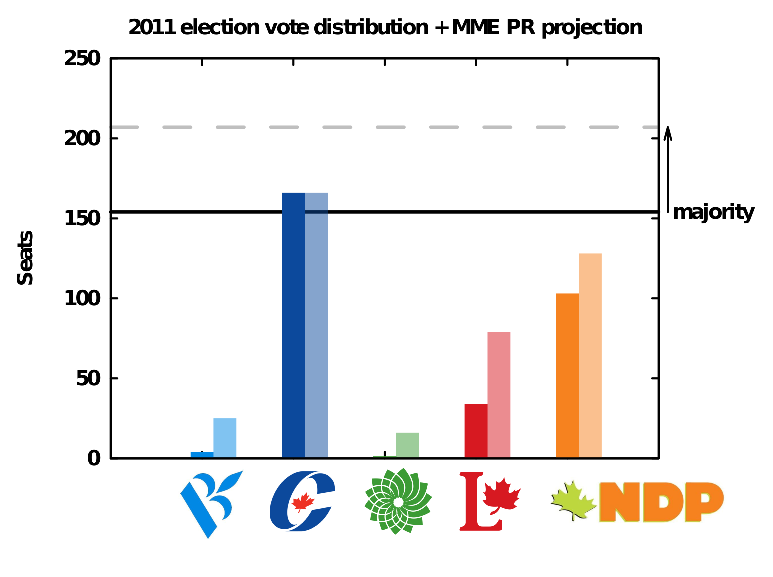
\includegraphics[width=0.50\textwidth,clip]{Figs/Osberg_PR_2011}
  \caption{ Seat distribution following the 2011 federal election for the major national parties. The solid and transparent bars correspond to the actual seat counts from the FPP system, and the hypothetical MMM projections respectively. The threshold for a majority government (solid bar) is shifted upwards to the dashed line as the total number of seats grows. 
}
\label{fig:hypo_2011}
\end{figure}

Likewise, Fig.~\ref{fig:hypo_2015} shows the same calculation for the 2015 election.

\begin{figure}[h!]
  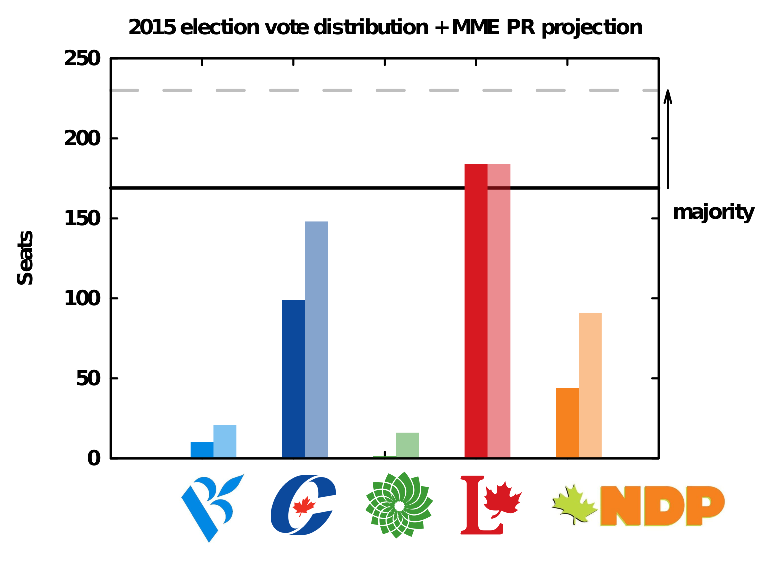
\includegraphics[width=0.50\textwidth,clip]{Figs/Osberg_PR_2015}
  \caption{ Seat distribution following the 2015 federal election, using the same conventions as in Fig.~\ref{fig:hypo_2011}.}
\label{fig:hypo_2015}
\end{figure}
It should be noted that there is nothing about this system that inherently prevents majority governments \--a party's lead could in fact be \emph{increased} into a majority with the second-ballot results. However, in practice, most governments with some form of PR have shown a tendency towards coalitions. Germany, for example, has established coalition governments as the norm in recent decades \---a historical trend that is evidently compatible with  stability.


%====================================================
\section{conclusion}	

There are many forms that electoral reform can take, and the right choice depends on defining the criteria for success, as I have attempted to do in Sec.~\ref{sec:goal_list}. The STV/ranked ballot satisfies enough of the criteria to merit serious consideration, and yet the German model comes even closer. 
The remaining flaws within the latter can be rectified by minimizing the number of additional MPs brought into place for proportionality by truncating the D'Hondt method, and by ensuring that the list of candidates who assume their positions for the sake of proportionality are pooled from a list ranked by popular vote (share) in their constituency. 

By implementing these changes, all MPs in parliament will have been through at least some formal filter of direct voter consultation and only the more popular members will represent their party in the house of commons; The number of additional MPs brought into place \--and, thus, the level of change to the existing system\-- is minimized; the  personal accountability between every voter and a representative is maintained; the voting mechanics are easily understood; MPs are supplied with a clearer mandate, and every vote will count.
Canada should adopt MMM. 

%----------------------------------------------------------------------------------------
%	REFERENCE LIST
%----------------------------------------------------------------------------------------

\begin{thebibliography}{99} % Bibliography - this is intentionally simple in this template

\bibitem{Broadbent_poll}
David Coletto and Maciej Czop,
{\color{blue} \href{https://d3n8a8pro7vhmx.cloudfront.net/broadbent/pages/4770/attachments/original/1448994262/Canadian_Electoral_Reform_-_Report.pdf?1448994262}{Canadian Electoral Reform}},
{\emph{Public Opinion on Possible Alternatives} }, December 2015

\bibitem{Leadnow_environics}
Environics,
{\color{blue} \href{http://www.votetogether.ca/pages/localpolling/}{`13 Swing Riding Polls - Wave One'}}, August 19, 2015

\bibitem{Blais}
Andre Blais and Kenneth Carty, 
`Does Proportional Representation Foster Voter Turnout?'
European Journal of Political Research 18(2):167 - 181 · May 2006

\bibitem{NZ_PR_results}
Jeffrey A. Karp and Susan A. Banducci
{\color{blue} \href{http://www.jkarp.com/pdf/ajps_1999.pdf}{`The Impact of Proportional Representation on Turnout: Evidence from New Zealand.'}},
{ \emph{Australian Journal of Political Science} }, \textbf{34},3,363-377

  
 \bibitem{Die_Zeit_negative_vote}
{\color{blue} \href{http://www.zeit.de/2005/39/Wahl\_paradox}{`Viele Farben, keine Wahl'}},
 { \emph{Die Zeit} }, September 22, 2005

\bibitem{Lakeman}
E. Lakeman,
{ \emph{Power to Elect} }, Suffolk, U.K.: The Electoral Reform Society (1982) pp 59-63.

\bibitem{Record}
 Michael Taube
{\color{blue} \href{http://www.therecord.com/opinion-story/6692466-liberals-electoral-reform-would-stack-the-deck-in-their-favour/}{ \emph{Liberals electoral reform would stack the deck in their favour} } },
Waterloo Region Record, May 27, 2016 

\bibitem{Stratmann}
Thomas Strattman
{\color{blue} \href{http://www.gmu.edu/centers/publicchoice/faculty%20pages/stratmann/vitae%20files/bunddev.pdf}{Party-Line Voting and Committee Assignments in the German Mixed Member System}}
Department of Economics, George Mason University

\bibitem{Irish_howto_vote_doc}
Department of the Environment, Community and Local Government, Ireland
{\color{blue} \href{http://www.environ.ie/sites/default/files/publications/files/guide_to_ireland_pr-stv_system_0.pdf}{A Guide to Ireland?s PR-STV Voting System}}
 
\end{thebibliography}

%====================================================
\clearpage
\section{Appendix}

When engineering a proportional adjustment to an existing set of constituent representatives, part of the difficulty stems from the fact that there is no fair or practical way of \emph{removing} representatives from parties that are over-represented. 
However, this need not necessarily interfere with proportionality. As stated above, the method used in this text is based around the D'Hondt highest averages method; we briefly review that now. 

For a parliament of size $N$ total seats, quotients $Q_{m,s}$ for each party $m$ are defined as 

\begin{equation}
\label{eq:Dhondt}
Q_{m,s} = \frac{V_m}{s +1},
\end{equation}
where $V_m$ is the number of votes won by party $m$  (out of a total of $\bar{V}$ second ballots), and $s$ is an index. In this method, $s$ is typically expanded from zero up to the number of seats in the house; each party obtains a list of such quotients, and the largest $N$ quotients are awarded seats. This method ensures that all parties obtain representation in proportion to their share of the popular vote. 
The difference between the usual D'Hondt method and the method employed here is that $N$ is not fixed. The value of $N$ is chosen to just accommodate all existing constituent representatives.

Let $C_m$ represent the number of direct constituent seats that party $m$ was awarded from the total $N^0$,
\begin{equation}
\label{eq:sum_Cm}
\sum_m C_m = N^0.
\end{equation}

Each party is then awarded a number of supplementary seats $D_m$ to establish their total seat count 

\begin{equation}
\label{eq:seat_total}
S_m=C_m+D_m.
\end{equation}

Together, these seats make up the whole parliament which will ultimately have size $N$
\begin{equation}
\label{eq:sum_Sm}
\sum_m S_m = N \ge N^0.
\end{equation}


We define the $m=0$ index to refer to the most initially over-represented party; that is, the party whose share of seats exceeds its share of popular votes by the largest margin:
\begin{equation}
\frac{C_0/N^0}{V_0/\bar{V}} \ge \frac{C_m/N^0}{V_m/\bar{V}} \,\, \,\,\,\, \forall \,\, m \neq 0.
\end{equation}
Extracting the common factor $N^0/\bar{V}$ reduces this to:
\begin{equation}
\label{eq:most_overrep}
\frac{C_0}{V_0} \ge \frac{C_m}{V_m} \,\, \,\,\,\, \forall \,\, m.
\end{equation}

Note that we have not \emph{explicitly} excluded ballots that were either spoiled or assigned to a party that fell below the 5\% threshold. Whether each voter should have their vote recognized in proportion to the whole of the voting population (including spoiled ballots) or only the number of valid votes is somewhat subjective. In this approach, spoiled ballots (and those cast for parties falling below the 5\% threshold) are implicitly excluded.

%This way, even spoiled ballots should still `count' in the sense that they broaden the pool of total votes from which other valid votes are compared to in proportion. In general, the greater the number of spoiled ballots, the fewer additional supplementary seats are required.

For each party, a list of quotients is defined in decreasing order
\begin{equation}
\label{eq:Qm_def}
\left\{ Q_m \right\} = V_m \, , \, \frac{V_m}{2} \, , \, \frac{V_m}{3} \ldots,
\end{equation}
and in general, party $m$'s $j-$th quotient is given by
\begin{equation}
\label{eq:Qmj_def}
Q_{m,j} = \frac{V_m}{j}.
\end{equation}

We may then combine these quotients from all eligible parties into the \emph{entire} list of quotients $\bar Q$, in decreasing order. As an example, we might imagine $\bar Q$ to look something like this.

\begin{equation}
\label{eq:Qbar_def}
\bar Q:  \left. Q_{0,1} > Q_{1,1} > Q_{2,1} >  Q_{0,2} > \ldots  Q_{0,C_0}  \right| Q_{n,S_{n}+1} \ldots 
\end{equation}
Notice the vertical bar to the right of the $Q_{0,C_0}$ term; each term to the left of this point corresponds to a seat in parliament. Each term to the right corresponds to a seat that is neither necessary to represent a constituency nor to establish proportionality, as such it is ignored.

How can we be sure of the latter claim? For each other party $m\neq 0$ we can see that $Q_{m,S_{m}}$ is, by definition, still to the left of this sequence termination, while $Q_{m,S_{m}+1}$ is to the right; in other words:
\begin{equation}
\label{eq:Qm_cutoff}
Q_{m,S_{m}}  > Q_{0,C_0} > Q_{m,S_{m}+1}. 
\end{equation}

Using the definition of $Q_m$, 
\begin{equation}
\label{eq:Sm_cutoff}
\frac{V_{m}}{C_{m}+D_m} \ge \frac{V_{0}}{C_0} \ge \frac{V_{m}}{C_{m}+D_m+1}\, , \,\, \forall \,\,  m. 
\end{equation}

Rearranging this expression establishes that the number of supplementary seats assigned to each party, $D_m$, is the largest integer that satisfies:
\begin{equation}
\label{eq:Dm_def}
D_m < \frac{ C_0 V_m - C_m V_0}{V_0},
\end{equation}
and
\begin{equation}
\label{eq:prop}
\frac{D_{m}+C_m}{V_{m}} \le \frac{C_0}{V_0} \, , \,\, \forall \,\, m. 
\end{equation}

Eq.~\ref{eq:Dm_def} gives a prescription for the number of seats to be added to each party's caucus $D_m$, while Eq.~\ref{eq:prop} establishes that the ratio of valid second-ballot votes received by each party to its number of seats is equal \---to the nearest integer. The party that obtains the final seat from the quotient $C_0/V_0$ (i.e. party $m=0$, which gained the greatest advantage from constituent seats) still wins the benefit of rounding.

%-------- COMMMNTED OUT THIS STUFF... MIGHT BRING IT BACK IN....--------------------
%\subsection{A simple worked example}
%Suppose party $X$ has $Q_0$ corresponding to the number of second-ballot votes for $X$ (divided by 1), $Q_1$ corresponding its second ballot votes divided by 2, $Q_2$ divided by three, etc.\ldots. 
%Parties $Y$ and $Z$ each have similar lists. All of these quotients are then assembled into one large list and ranked by size from largest to smallest. 
%In the standard D'Hondt method, if there are $N$ seats in the assembly, then the first $N$ quotients are converted to seats. 
%
%Thus, for example, if 15 of those $N$ largest quotients came from party $X$'s list, then party $X$ will be awarded 15 candidates in parliament. This establishes proportionality to the nearest integer number of seats for each party.
%
%
%
%If 15 of those $N$ largest quotients came from party $X$'s list, then party $X$ will be awarded 15 candidates in parliament. This establishes proportionality to the nearest integer number of seats for each party.
%
%Here is where we differ from the standard D'Hondt method: there is no reason $N$ must be fixed in size prior to the calculation \---we may adjust this number to be just as large as necessary to capture all of the existing constituency representatives from each party. Proportionality naturally arises wherever we draw the line along this list, and the minimum number of additional candidates necessary for proportionality will simply be bundled in.
% 
% To see this in practice, suppose party $Y$ is the most over-represented party from constituency elections (ballot 1) with 60 seats out of 100, despite winning only 40\% of the public support (from ballot 2). The underrepresented parties $X$ and $Z$ are then entitled to more seats for proportionality, and we must calculate how many.
%
%As the list of quotients from formula \ref{eq:DHondt_app}  is read through, all three parties can be assigned seats, and initially, we may merely ascribe these seats to the constituency-winners who have already been elected from ballot 1.
%
%Eventually, however, one or both of parties $X$ and $Z$ will exhaust their constituency candidates and require `top-ups'. 
%This is the point at which supplementary MPs (using terminology from the main text) are pooled from the candidate list based on vote share from their constituency. 
%The process will then continue until eventually the most initially over-represented party has had its full complement of constituency winners accounted for. In our example, this is when  party $Y$ is awarded its 60H seat. At this point the whole process stops immediately, the quotient expansion is truncated and the result, down to this point, is the next governing parliament. In real examples, from the 2011 national election this occurred when the Conservative Party of Canada was awarded its 166th seat, while in 2015 this corresponds to the Liberal Party of Canada's 184th seat. 

To reiterate, the process is as follows:
\begin{enumerate}
\item Determine the most over-represented party from the constituency contests and its direct constituency seat count (as an example, suppose this is party $Z$ with 60 constituent seats.)
\item Expand the quotient list (Eq.~\ref{eq:Qbar_def}) by combining the quotients from each party (Eq.~\ref{eq:Qm_def}), with each term ordered by size, and distribute seats to the ranked list of quotients in order as per the usual D'Hondt method. 
\item This process will assign a mix of supplementary MPs and MPs already based from constituencies from other party lists (e.g. $X$ and $Y$) until party $Z$'s constituent list is exhausted (in this example, when party $Z$ is awarded its 60th seat). All constituent MPs from parties $X$ and $Y$ will have then been seated along with the minimum necessary number of additional seats needed to establish proportionality. Seat allocation is then complete.
\end{enumerate}

Data from recent elections indicates that this process would be sufficient to establish a representative parliament with minimal expansion (see Figs.~\ref{fig:hypo_2011},\ref{fig:hypo_2015}), however, we can imagine pathological cases. 

Let us take the most extreme possible example as a thought experiment: suppose the under-represented party in our example, $X$, receives zero \---or few\--- constituency seats, and yet is awarded 100\% of the second-ballot votes (this is, of course, exceedingly unlikely in practical terms, but theoretically possible, since the model allows for voters to choose between candidate and party independently). 
A truly proportional legislature in this case would require adding an \emph{infinite} number of representatives from party \textbf{$X$} \---an obviously impractical conclusion. For this reason, an additional \--and somewhat subjective\-- clause is necessary: parliament may never reach more than a maximum upper limit which I will define as $\hat N$. Whereas in the German system, $N$ is always  twice the number of constituencies, in our model, this quantity $\hat N = 2 N^0$ is set as our upper-limit to ensure that constituent MPs are never in the minority, although more conservative constraints (i.e. smaller values of $\hat N$) are also possible. The general rule remains:

\begin{equation}
\label{eq:Nlimits}
N^0 \le N \le \hat N.
\end{equation}


When reading down the list in Eq.~\ref{eq:Qbar_def} above, when the number of remaining seats available  reaches the number of direct constituency seats not yet accounted for, then these constituency candidates are automatically admitted, regardless of ordering. In practice, one could equivalently think of this as excluding those $N^0$ seats from the list in Eq.~\ref{eq:Qbar_def} and reading only $\hat N - N^0$ seats from left to right from the remainder. 

Although underrepresentation of certain parties could still remain, this would be unlikely, in practice, and if all $\hat N$ seats are exhausted, the prospect of a single party maintaining a majority would be fantastically improbable.

A somewhat more plausible scenario (though still quite unlikely) would be if a single party's list of constituent representatives is exhausted. From this point, the party would have to choose further nominees itself.

This potential deviation from proportionality is a kind of safety mechanism to avoid enormous parliament sizes, but in practice would only be necessary in unusual cases (neither the 2011 nor 2015 results nearly approach this kind of behavior, though an exhaustive study of when such a historical case might have been observed has not been conducted).

Another possible formula for calculation is presented below
%============================================================
\subsection{An Alternative (Compromise) Formula}

There is an alternative method of awarding seats to under-represented parties that is somewhat of a compromise between perfect proportionality and the current FPP system. To introduce this, we use the Droop quota from the Irish STV, defined as:

\begin{equation}
\label{eq:Droop_def}
Q_{ \textrm{Droop} } =\frac{ \left( \textrm{Total} \,\, \textrm{Votes} \right)}{ \left( \textrm{Seats} \,+1\right)} +1,
\end{equation}

which serves as a kind of conversion between votes and seats. Thus, if party $X$ wins a number of second-ballot votes equal to 34.7 times the Droop quota, then it ought to have been awarded 34 seats in parliament (rounding down). If it received only 30 seats in constituency races, then one might argue that it is `owed' 4 seats. 
True proportionality would require also \emph{removing} 4 seats from another party, but as we've established above, that isn't feasible. 
One approximate solution would be to simply neglect this effective `dilution' factor. 

To clarify, the Droop quota itself in Eq.~\ref{eq:Droop_def} is defined in terms of the total number of seats. As the number of seats is increased, this value changes. However, one might simplify the calculation by neglecting this change and keeping the Droop quota constant regardless. 
This would imply that representatives added to the party \textbf{$X$} caucus now occupy a slightly smaller fraction of this enlarged parliament, but it would also have the benefit of automatically ensuring that parliament is never more than doubled in size. 

In most realistic scenarios, the decision to keep the quota constant, rather than using the more precise method in the previous section, makes little difference \---as a crude analogy, one might say that restoring a party's proportional seats in this manner is like repaying the principal of a loan without the interest. 

In the two examples provided in the text (from the 2011 and 2015 national elections) the most that any political party remained under-represented after this procedure was a 4\% difference between popular vote share and seat distribution using this formula \---down from about 10\% prior to this adjustment. 

\begin{figure}[h!]
  \includegraphics[width=0.50\textwidth,clip]{Figs/PR_Droop_2011_output}
  \caption{ Seat projection following the 2011 federal election, using the `compromise' algorithm from Eq.~\ref{eq:Droop_def}. Fewer seats are added to the constituent base, and proportionality is approached but not reached exactly.}
\label{fig:Droop_2011}
\end{figure}

\begin{figure}[h!]
  \includegraphics[width=0.50\textwidth,clip]{Figs/PR_Droop_2015_output}
  \caption{ The same projection as Fig.~\ref{fig:Droop_2011}, using data from the 2015 national election.}
\label{fig:Droop_2015}
\end{figure}

Larger deviations are possible, however, as we saw in the hypothetical extreme case above where party \textbf{$X$} earned 100\% of the popular vote on the second ballot with no direct constituency wins. In this case, $X$ will naturally  be assigned 50\% of the seats.

It may be argued that our goal is to \emph{approximate} proportionality, in order to provide some mechanism of restoring representation to parties that were strongly disfavored by delegate math or gerrymandering. This is perhaps sufficient to minimize the disenfranchisement felt by voters at \emph{large} disparities between popular support and representation. 
Ultimately, in this solution however, the importance of winning in local ridings is not completely obviated; it may be a palatable compromise.

%----------------------------------------------------------------------------------------

\end{document}
